\documentclass[aspectratio=169, dvipdfmx, 11pt, uplatex]{beamer}

% 日本語対応
\usepackage{bxdpx-beamer}
\usepackage{pxjahyper}
\usepackage{minijs}

% 数式・図表
\usepackage{amsmath,amssymb,bm,mathtools}
\usepackage{graphicx}
\usepackage{booktabs}
\usepackage{tikz}

% BibLaTeX
\usepackage[
    citestyle=authoryear-comp,
    bibstyle=authoryear-comp,
    maxcitenames=3,
    backend=biber,
    style=authoryear
]{biblatex}
\addbibresource{literature.bib}
\setbeamertemplate{bibliography item}{}

\renewbibmacro{in:}{}
\DeclareFieldFormat{url}{\url{#1}}

\setbeamercolor{bibliography entry author}{fg=black}
\setbeamercolor{bibliography entry title}{fg=black}
\setbeamercolor{bibliography entry location}{fg=black}
\setbeamercolor{bibliography entry note}{fg=black}
\hypersetup{
    colorlinks=true,
    linkcolor=black,
    citecolor=black,
    urlcolor=blue
}

% テーマ
\usetheme{Boadilla}
\usefonttheme{professionalfonts}

% 日本語フォント（ゴシック標準）
\renewcommand{\kanjifamilydefault}{\gtdefault}

% 色（必要最小限）
\newcommand{\red}[1]{\textcolor{red}{#1}}
\newcommand{\blue}[1]{\textcolor{blue!80!black}{#1}}

% リンク
\hypersetup{
    colorlinks=true,
    linkcolor=blue,
    citecolor=blue
}

% ナビゲーション削除
\setbeamertemplate{navigation symbols}{}

% ページ番号のみ（少し上・大きめ）
\setbeamertemplate{footline}{
  \hfill
  \raisebox{2mm}{
    \usebeamerfont{page number in head/foot}
    \fontsize{16}{18}\selectfont
    \insertframenumber
  }
  \hspace{1em}
}

% itemize（軽く調整）
\setbeamertemplate{itemize item}{\small$\bullet$}
\setbeamertemplate{itemize subitem}{\tiny$\blacktriangleright$}
\setbeamertemplate{enumerate item}{\arabic{enumi}.}
\setbeamertemplate{enumerate subitem}{\arabic{enumii}.}
% --------------------
% Overall information
% --------------------
\title{
【卒論 経過報告】 \\
\vspace{5mm}
総量規制はバブル崩壊を引き起こしたのか？ \\
～モデル・シミュレーション・VAR分析～
}
\date{Ver.1. 2026.5.11 \\
Ver.2. 2026.5.12
}
\author{岸本康佑}
\institute{
東洋大学 経済学部 経済学科 4年 \\
\texttt{s12102301404@toyo.jp}, \texttt{kishimoto.research@gmail.com} \\
GitHub: https://github.com/Kishimoto-econ
}


\begin{document}

\begin{frame}
  \titlepage
\end{frame}


\begin{frame}{目次}
  \begin{columns}[t]
    \begin{column}{0.48\textwidth}
      \tableofcontents[sections={1-4}]
    \end{column}
    \begin{column}{0.48\textwidth}
      \tableofcontents[sections={5-9}]
    \end{column}
  \end{columns}
\end{frame}

\section{研究課題}
\begin{frame}{研究課題}
  \begin{itemize}
    \item 本研究では，バブル期の1990年代に地価抑制政策として実施された土地関連融資の規制，いわゆる「総量規制」が地価下落やバブル崩壊を招いたかをDSGEモデルを用いて分析する
    \item 総量規制が地価下落やバブル崩壊に大きく影響したという主張は，当時の業界関係者によるオーラル・ヒストリーで語られる事が多く，一般的な通説となっている（例えば，\textcite{I2011}）
    \item しかし，理論的・実証的な研究は数が少なく，学問的なコンセンサスが取れているとは言い難い
    \item その理由として，\textcite{U2012}が指摘するように，総量規制が地価や生産量に与える影響を明示的に捉えることが困難であることが挙げられる
    \item そこで，本研究では，「不況の増幅メカニズム」を理論的に明らかにした\textcite{KM1997}を用いて，総量規制が地価や生産量に影響を与えるメカニズムを示したうえで，実際のデータを使って分析を行う
    \item 本研究によって，バブル崩壊の経済史的な発見だけでなく，不動産バブルへの対応に関する政策インプリケーションやLTV規制といったマクロ・プルーデンス政策につながる発見が得られる可能性がある
  \end{itemize}
\end{frame}

\section{モデルのイメージ図}
\subsection{静学的メカニズム}
\begin{frame}{モデルのイメージ：$t$期} \label{image1}
\begin{figure}
    \begin{minipage}{0.55\linewidth}
        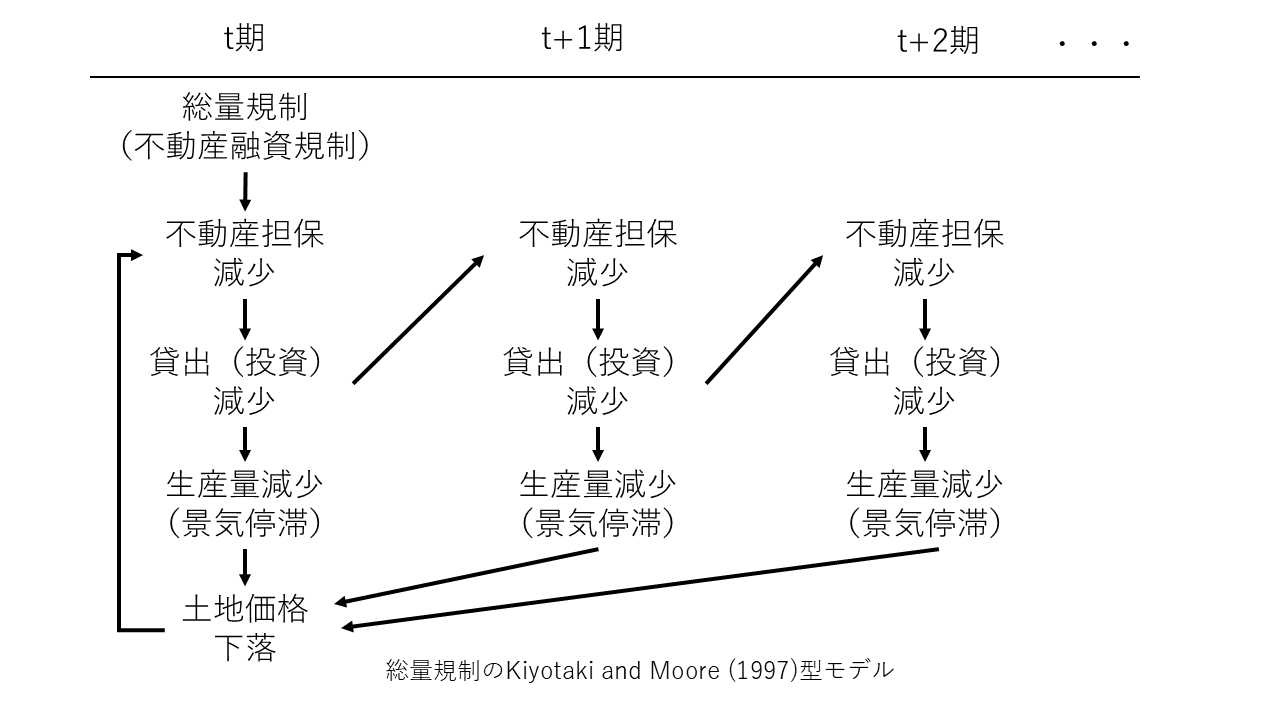
\includegraphics[width=1.15\linewidth]{model_image.png}
    \end{minipage}
    \begin{minipage}{0.4\linewidth}
        \begin{enumerate}
        \item 総量規制は「不動産融資の伸び率」を「他の融資の伸び率」よりも小さくする規制
        \item 不動産融資が減少すると，不動産の購入が減り，担保は減少
        \item 担保が減少すると，銀行は貸出を抑える（=投資は減る）
        \item 貸出（投資）が減少すると，生産量は減少し，景気は停滞する
        \item 景気が停滞すると，土地価格は下落する
        \item 土地価格が下落すると，担保価値が下落する
        \item 以下，同じ期内でこのループが繰り返される
        \end{enumerate}
    \end{minipage}
\end{figure}
\end{frame}

\subsection{動学的メカニズム}
\begin{frame}{モデルのイメージ：$t$期，$t+1$期，$t+2$期，・・・} \label{image2}
\begin{figure}
    \begin{minipage}{0.55\linewidth}
        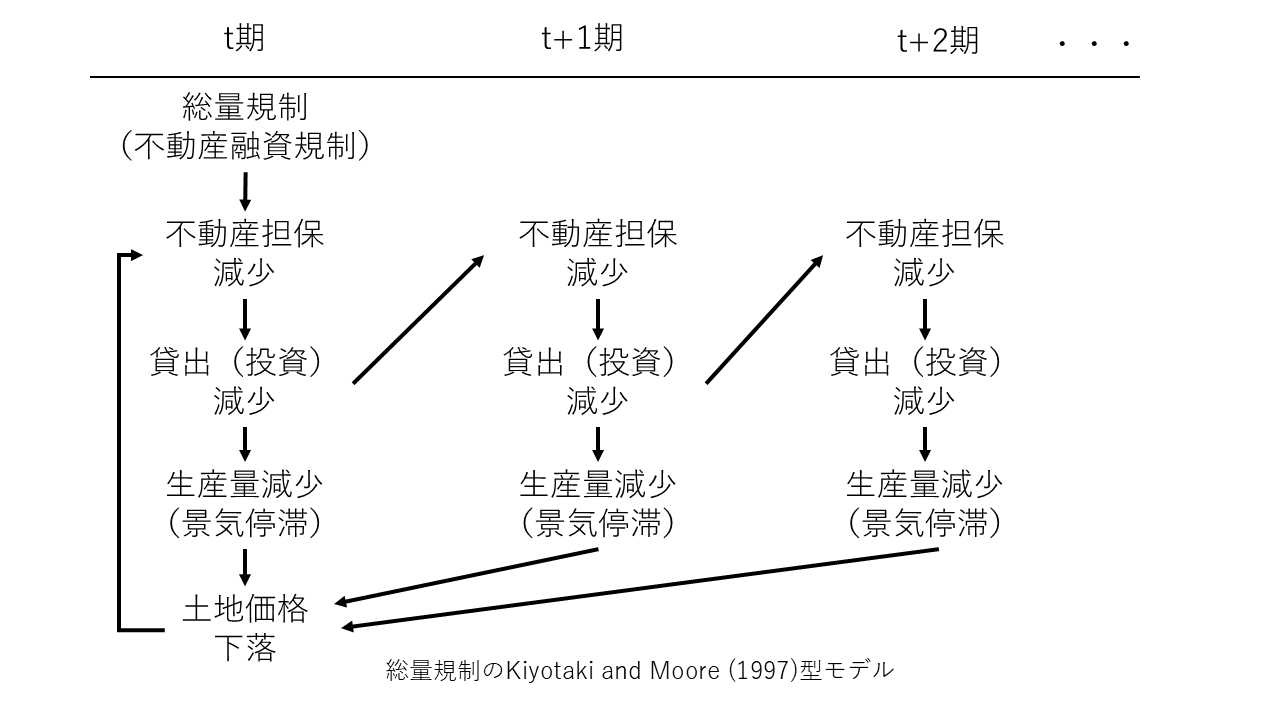
\includegraphics[width=1.15\linewidth]{model_image.png}
    \end{minipage}
    \begin{minipage}{0.4\linewidth}
        \begin{enumerate}
          \item $t$期での貸出（投資）減少は，$t+1$期での不動産担保を減少させる
          \item 以下，$t$期と同様に「不動産担保減少⇒貸出減少⇒生産量減少⇒土地価格下落」が起きる
          \item $t+1$期から$t+2$期，それ以降についても同様である
        \end{enumerate}
        \begin{itemize}
          \item 一時的な政策であった総量規制が，動学メカニズムによってその効果が増幅され，バブル崩壊を招いた可能性をモデル化
          \item 合理的期待と担保制約を組み込んだ\textcite{KM1997}を用いることで分析可能に
        \end{itemize}
    \end{minipage}
\end{figure}
\end{frame}

\section{\textcite{KM1997}の概要}

\begin{frame}{\textcite{KM1997}の概要}
以下の説明は\textcite{S2020}，\textcite{W2010}を参考にした
  \begin{itemize}
    \item \textcite{KM1997}は，経済主体をFamerとGathererの2つに分ける
    \item 財もtradableな財と，not-tradableだが生産者（Farmer）の自家消費が可能な財の2財に分ける
  \end{itemize}
  \begin{description}
    \item[Farmer] \mbox{} \\
      \begin{itemize}
        \item 保有する土地$k_t$を使って生産を行い，さらに土地を担保にしてGathererから借入$b_t$を行う \\
        \item 生産関数は$y_{t+1}=(a+c)k_t$（$ak_t$：tradable output，$ck_t$：not-tradableだが自家消費可能なoutput） \\
        \item \textcolor{blue}{来期の土地価値$q_{t+1} k_t$を担保にした借入制約がある}：$R_t b_t \leq q_{t+1} k_t$（$R_t$：金利，$b_t$：借入金，$q_{t+1}$：土地価格） \\
        \item 自家消費分$ck_{t}$以上の消費をする：$x_t \geq c k_{t-1}$
      \end{itemize}
    \item[Gatherer] \mbox{} \\
      \begin{itemize}
        \item 保有する土地$k'_t$を使って生産を行う \\
        \item 生産関数は$y'_{t-1}=G(k'_t), where \, G'>0, G''<0, G'(0)>aR>G'(\frac{\bar{K}}{m})$
      \end{itemize} 
  \end{description}
\end{frame}

\subsection{Farmerの行動}
\begin{frame}{Farmerの行動：定式化}
  Farmerの行動は以下の効用最大化問題の解として定式化できる
  \begin{align}
    \max_{x_t, b_t, k_t, q_t} \quad & \mathbb{E}_t \bigg( \sum_{s=0}^{\infty} \beta^s x_{t+s} \bigg) \label{eq:f_u} \\
\text{s.t.} \quad & q_t(k_t - k_{t-1}) + R b_{t-1} + x_t - c k_{t-1} = a k_{t-1} + b_t \label{eq:f_yosan} \\
& R b_t \leq q_{t+1} k_t \label{eq:kariire}\\
& x_t \geq c k_{t-1} \label{eq:syouhi}
  \end{align}
  \begin{itemize}
    \item \eqref{eq:f_u}式は，消費$x_t$の割引現在価値の合計であり，Farmerの効用関数
    \item \eqref{eq:f_yosan}式は，左辺第1項が土地購入費用，第2項が借入金の返済，$x_t-ck_{t-1}$が自家消費分の生産を超えた消費，右辺が生産と借入による収入を表す予算制約式
    \item \eqref{eq:kariire}式は土地価値$q_{t+1} k_t$を超えて，金利を含めた借入$R b_t$ができないという借入制約
    \item \eqref{eq:syouhi}式はnot-tradable output以上の消費$x_t$をするという消費制約
  \end{itemize}
\end{frame}

\begin{frame}{Farmerの行動：最適化}
  \begin{itemize}
    \item Farmerの効用最大化問題のラグランジアンは以下の通り
      \begin{equation}
        \begin{aligned}
          \mathcal{L} = \mathbb{E}_0 \sum_{s=0}^{\infty} \beta^s \bigg[ & x_{t+s} + \lambda_{t+s} [(a + c) k_{t+s-1} + b_{t+s} - q_{t+s} (k_{t+s} - k_{t+s-1}) \\
          &- R b_{t+s-1} - x_{t+s}] \\
          &+\mu_{t+s}[q_{t+s+1}k_{t+s} - R b_{t+s}] + \varphi_{t+s}[x_{t+s} - ck_{t+s-1}] \bigg]
        \end{aligned}
      \end{equation}
    \item 効用最大化の1階条件を導出する
      \begin{align}
        &\frac{\partial\mathcal{L}}{\partial x_t}: 1 - \lambda_t + \varphi_t = 0 \\
        &\frac{\partial\mathcal{L}}{\partial b_t}: \lambda_t - \mu_t R + \beta \lambda_{t+1} R = 0 \\
        &\frac{\partial\mathcal{L}}{\partial k_t}: - q_t \lambda_t + \mu_t q_{t+1} + \beta \lambda_{t+1}[(a+c) + q_{t+1}] - \beta c \varphi_{t+1} = 0
      \end{align}
  \end{itemize}  
\end{frame}

\begin{frame}{Farmerの行動：最適化}
  \begin{itemize}
    \item 上記の1階条件より，消費制約と土地価格のオイラー方程式を得る
      \begin{align}
        1 + \varphi_t &= (\beta(1+\varphi_{t+1}) + \mu_t) R \\
        q_t (1 + \varphi_t) + \beta c \varphi_{t+1} &= \beta(1 + \varphi_{t+1})[a + c + q_{t+1}] + \mu_t q_{t+1}
      \end{align}
  \end{itemize}
\end{frame}

\subsection{Gathererの行動}
\begin{frame}{Gathererの行動：定式化}
  Gahtererの行動は以下の効用最大化問題の解として定式化できる
  \begin{align}
    \max_{x'_t, b'_t, k'_t, q_t} \quad & \mathbb{E}_t \bigg( \sum_{s=0}^{\infty} \beta'^s x'_{t+s} \bigg) \label{eq:g_u} \\
\text{s.t.} \quad & q'_t(k'_t - k'_{t-1}) + R b'_{t-1} + x'_t = G(k'_{t-1}) + b'_t \label{eq:g_yosan}
  \end{align}
  \begin{itemize}
    \item \eqref{eq:g_u}式は，消費$x'_t$の割引現在価値の合計であり，Gathererの効用関数
    \item \eqref{eq:g_yosan}式は，左辺第1項が土地購入費用，第2項が借入の返済，第3項が消費，右辺が生産と借入による収入を表す予算制約式
    \item 定常状態では，Gathererは貸し手側なので$b'_t < 0$，すなわち左辺第2項は貸した資金の返済である
  \end{itemize}
\end{frame}

\begin{frame}{Gathererの行動：最適化}
  \begin{itemize}
    \item Gathererの効用最大化問題のラグランジアンは以下の通り
      \begin{equation}
        \begin{aligned}
          \mathcal{L} = \mathbb{E}_0 \sum_{s=0}^{\infty} \beta'^s \bigg[ & x'_{t+s} + \lambda'_{t+s} [G(k'_{t+s-1}) + b'_{t+s} - q_{t+s} (k'_{t+s} - k'_{t+s-1} - R b'_{t+s-1} - x'_{t+s}] \bigg]
        \end{aligned}
      \end{equation}
    \item 効用最大化の1階条件を導出する
      \begin{align}
        \frac{\partial \mathcal{L}}{\partial x_t'} &: 1 - \lambda_t' = 0 \\
        \frac{\partial \mathcal{L}}{\partial b_t'} &: \lambda_t' - \beta' R_t \lambda_{t+1}' = 0 \\
        \frac{\partial \mathcal{L}}{\partial k_t'} &: -\lambda_t' q_t + \beta \lambda_{t+1}' G'(k_t') + \beta q_{t+1} = 0
      \end{align}
    \item 名目金利$R$の定義式と土地価格$q_t$のオイラー方程式を得る
      \begin{align}
        1 &= \beta' R \label{eq:rishi} \\
        q_t &= \beta' [G'(K'_t) + q_{t+1}]
      \end{align}
  \end{itemize}
\end{frame}

\subsection{モデルの全体像}
\begin{frame}{モデルの全体像}
  \begin{itemize}
    \item 以上より，\textcite{KM1997}のSection 2で構築されたモデルを連立差分方程式で表せるようになった
    \item Section 3では投資が導入された，より複雑なモデルが構築されているが今回の分析には必要ない
      \begin{gather}
        q_t(k_t - k_{t-1}) + \frac{1}{\beta'} b_{t-1} + x_t - c k_{t-1} = a k_{t-1} + b_t \label{eq:model1} \\
        b_t \leq \beta' q_{t+1} k_t \label{eq:model2} \\
        x_t \geq c k_{t-1} \\
        1 + \varphi_t = (\beta(1+\varphi_{t+1}) + \mu_t) \frac{1}{\beta'} \label{} \\
        q_t (1 + \varphi_t) + \beta c \varphi_{t+1} = \beta(1 + \varphi_{t+1})[a + c + q_{t+1}] + \mu_t q_{t+1} \\
        q_t = \beta' [G'(K'_t) + q_{t+1}] \\
      \end{gather}
  \end{itemize}
  （続く）
\end{frame}

\begin{frame}{モデルの全体像}
  （続いた）
  \begin{gather}
    x_t + m x'_t = (a + c) k_{t-1} + m G(K'_{t-1}) \label{eq:kinkou1} \\
    k_t + m k'_t = \bar{K} \label{eq:kinkou2}
  \end{gather}
  \begin{itemize}
    \item ただし，$b_t + m b'_t = 0$とした
    \item \eqref{eq:kinkou1}式，\eqref{eq:kinkou2}式は均衡条件式である
    \item \eqref{eq:kinkou1}式は総生産量であり$Y_t$とおく．また$\bar{K}$は定数である
    \item ここから定常状態の導出を行えばDynareでシミュレーションができる
    \item 正の生産性ショックが起きた場合のIRFは以下の通り（\textcite{P2025}のコードを使用）
      \begin{figure}
        \centering
        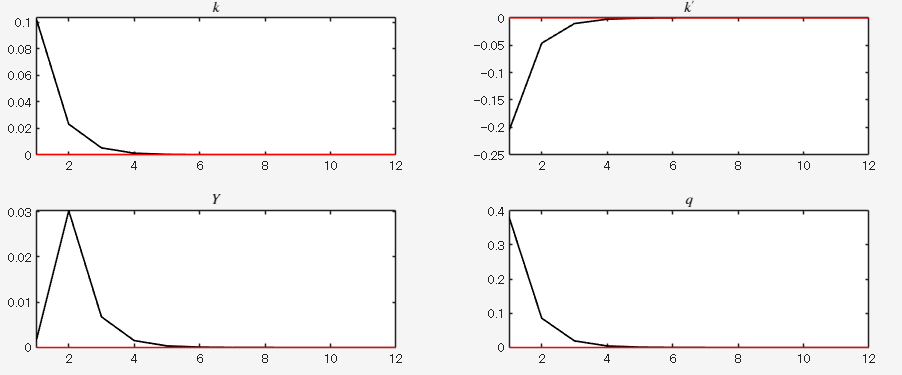
\includegraphics[width=0.5\linewidth]{kiyotaki_moore_1997.png}
      \end{figure}
  \end{itemize}
\end{frame}

\section{総量規制ショック}
\subsection{ショックの導入}
\begin{frame}{総量規制ショックの導入}
  \begin{itemize}
    \item ここからは\textcite{KM1997}に総量規制ショックを導入して，地価$q_t$や総生産量$Y_t$がどのように動くかをシミュレーションする
    \item 総量規制とは，不動産融資の伸び率を全体の融資の伸び率以下に抑えることを大蔵省が金融機関に求めた政策である
    \item しかし，不動産融資とその他の融資に分けることは，変数の増加やモデルを不必要に複雑にしてしまう
    \item そこで，総量規制は不動産投資を減少させる政策であるから，Farmerが所有する土地$k_t$に対する負のショックと捉える
    \item これにより，\textcite{KM1997}にFarmerの土地$k_t$へのショックを導入するだけで総量規制が地価$q_t$や総生産量$Y_t$に与える影響を分析できるようになった
  \end{itemize}
\end{frame}

\begin{frame}{$k_t$に対するショックの導入}
$k_t$に対するショックを$\varepsilon_t^k$とする \\
ただし，$\mathbb{E}_t \varepsilon_{t+j}^k = 0, \, for \, j > 0 \notag$かつ$iid$である
  \begin{itemize}
    \item \eqref{eq:model1}式より，
      \begin{equation}
        q_t(k_t (1+\varepsilon_t^k) - k_{t-1}) + \frac{1}{\beta'} b_{t-1} + x_t - c k_{t-1} = a k_{t-1} + b_t
      \end{equation}
    \item \eqref{eq:model2}式より，
      \begin{equation}
        b_t \leq \beta' q_{t+1} k_t (1+\varepsilon_t^k)
      \end{equation}
    \item \eqref{eq:kinkou2}式より，
      \begin{equation}
        k_t (1+\varepsilon_t^k) + m k'_t = \bar{K}
      \end{equation}
  \end{itemize}
\end{frame}

\subsection{シミュレーション}
\begin{frame}{総量規制ショックのシミュレーション}
  \begin{minipage}{0.55\linewidth}
    \begin{figure}
      \centering
      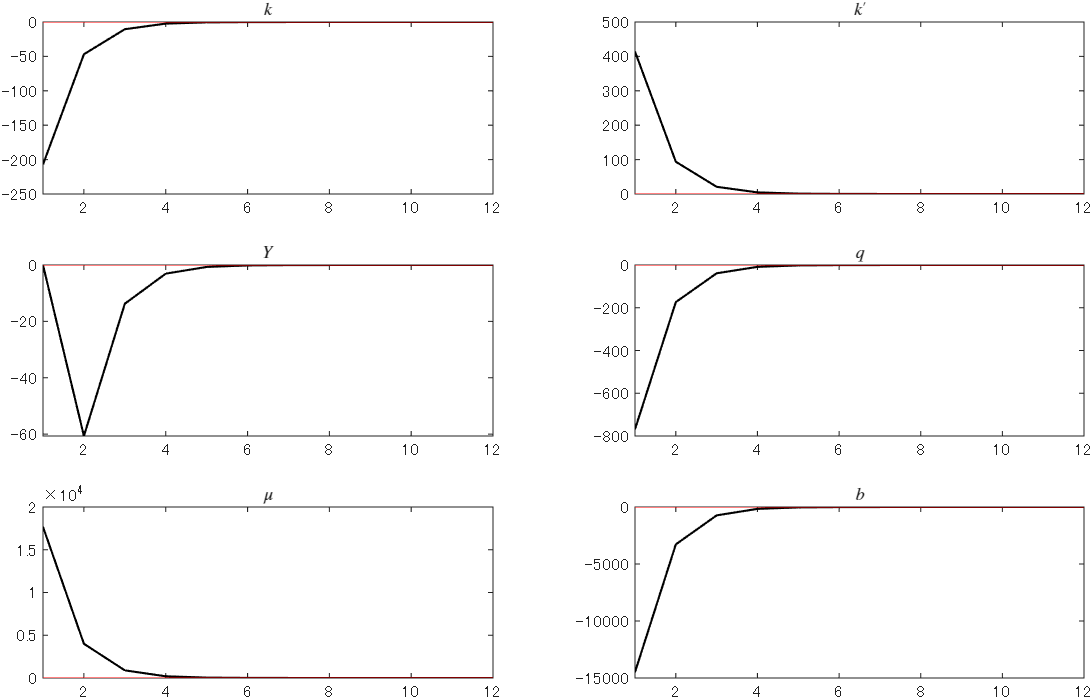
\includegraphics[width=1.0\linewidth]{kiyotaki_moore_1997_k.png}
    \end{figure}
  \end{minipage}
  \begin{minipage}{0.4\linewidth}
    \begin{itemize}
      \item 土地の総量は，$k_t + m k'_t = \bar{K}$で一定だから，$k_t$を減少させるショックは，$k'_t$を増加させる
      \item 借入$b_t$，総生産量$Y_t$，土地価格$q_t$すべてが減少している
      \item タイムラグを持った動きをしている
      \item \textcolor{blue}{総じて，スライド\ref{image1}，\ref{image2}の説明と同じ動きをしていると言える}
      \item ラグランジュ乗数$\mu_t$は借入制約の強さを意味し，増加しているが理由は今のところ分からない
    \end{itemize}
    \textcolor{red}{$Y$の動きが1期遅れているので修正が必要とのご指摘あり（5/11）}
  \end{minipage}

\end{frame}

\section{VAR分析}
\subsection{概要とデータの出典}
\begin{frame}{VAR分析：概要とデータの出典}
  \begin{itemize}
    \item モデルが現実の動きと一致しているかを調べるためにVAR分析を行った
    \item モデルに金融政策を導入するかもしれないので，名目金利$i$を加えている（結果はほぼ同じ）
    \item ショックの識別には，コレスキー分解を用いた
    \item \textcite{U2005}は\textcite{KM1997}をVAR分析で実証分析し，全体を十分説明する結果は得られなかったが，循環的な振る舞いの発生は観察されたとしている
  \end{itemize}
  \begin{description}
    \item[データの出典] \mbox{} \\
      \begin{itemize}
        \item データ期間は1980年第1半期から2007年第2半期までの半期データで，サンプル数は56である
        \item $b_t$：『法人企業統計調査』の当期末の「短期借入金計」と「長期借入金計」の合計
        \item $k_t$：『法人企業統計調査』の当期末固定資産の「土地」
        \item $q_t$：『市街地価格指数』（日本不動産研究所）の「全用途平均」
        \item $Y_t$：『実質国内総支出』
        \item $i_t$：『有担保コールレート・翌日物』
        \item $b_t$，$k_t$，$q_t$は\textcite{U2005}と同じデータの出典である（期間は異なる）
      \end{itemize}
  \end{description}
\end{frame}

\subsection{ADF検定}
\begin{frame}{VAR分析：ADF検定}
  \begin{itemize}
    \item データに単位根が含まれているかを調べるため，拡張ディッキー・フラー（ADF）検定を行った
    \item データは分散を標本期間内で均一にするため対数値に変換．$\Delta$は１階の階差をとったもの．*は有意水準10％，**は有意水準5％，***は有意水準1％
    \item 名目金利$i$はゼロ金利政策の期間を含むので検定を行っていない
  \end{itemize}
  \begin{description}
    \item[借入金$b_t$] \mbox{} \\
      \scalebox{0.8}{
        \begin{tabular}{cccc} \hline
            & 定数項およびトレンドなし & 定数項あり & 定数項およびトレンドあり \\ \hline
           $b$ & $0.3731$ & $-2.4219$ & $-0.4579$ \\
           $\Delta b$ & $-1.8209$* & $-1.5976$ & $-3.3411$* \\ \hline
        \end{tabular}}
      \item[Farmer保有の土地$k_t$] \mbox{} \\
        \scalebox{0.8}{
          \begin{tabular}{cccc} \hline
              & 定数項およびトレンドなし & 定数項あり & 定数項およびトレンドあり \\ \hline
             $k$ & $0.3018$ & $-10.5647$*** & $-2.5694$ \\
             $\Delta k$ & $-2.8381$*** & $-1.9890$ & $-10.4806$*** \\ \hline
          \end{tabular}}
      \item[土地価格$q_t$] \mbox{} \\
        \scalebox{0.8}{
          \begin{tabular}{cccc} \hline
              & 定数項およびトレンドなし & 定数項あり & 定数項およびトレンドあり \\ \hline
             $q$ & $0.1482$ & $-2.0385$ & $-0.3419$ \\
             $\Delta q$ & $-2.2902$** & $-2.2075$ & $-3.6911$** \\ \hline
          \end{tabular}}
  \end{description}
（続く）
\end{frame}

\begin{frame}{VAR分析：ADF検定}
（続いた）
  \begin{description}
    \item[総生産量$Y_t$] \mbox{} \\
      \scalebox{0.8}{
        \begin{tabular}{cccc} \hline
            & 定数項およびトレンドなし & 定数項あり & 定数項およびトレンドあり \\ \hline
           $Y$ & $0.6076$ & $-2.9130$** & $-2.9507$ \\
           $\Delta Y$ & $-1.4596$ & $-1.4300$ & $-2.2149$ \\ \hline
        \end{tabular}}
    \item[考察] \mbox{} \\
      \begin{itemize}
        \item 差分を取らない場合，すべての変数で非定常性の問題がある可能性がある
        \item 1階の差分を取った場合，総生産量$Y_t$以外の変数では改善が見られた
        \item よって，不十分ではあるが，すべての変数は１階の階差をとれば定常となると判断しVAR分析を行う
      \end{itemize}
  \end{description}
\end{frame}

\subsection{結果と考察}
\begin{frame}{VAR分析：結果}
  正の1標準偏差ショックに対するIRFは以下の通りである（負のショックは上下反転）
  \begin{figure}
    \centering
    
\includegraphics[scale=0.39]{var.png}
  \end{figure}
\end{frame}

\begin{frame}{VAR分析：考察}
以下はFarmerが保有する土地$k$の負のショックに対する考察である
  \begin{itemize}
    \item 借入金$b$は負に反応
      \begin{itemize}
        \item 不動産担保の減少が貸出を減少させる
      \end{itemize}
    \item 総生産量$Y$は負に反応
      \begin{itemize}
        \item 借入金（貸出）の減少によって，生産量が減少
      \end{itemize}
    \item 土地価格$q$は負に反応し，持続的
      \begin{itemize}
        \item 貸出減少による不動産需要の減退や景気停滞によって，土地価格は下落
        \item さらに土地価格の下落は長期間続く
      \end{itemize}
    \item 名目金利$i$は目立った反応を示さず
    \item \textcolor{blue}{総じて，スライド\ref{image1}，\ref{image2}の説明と同じ動きを説明していると言える}
  \end{itemize}
名目金利$i$の正のショック（公定歩合の引き上げ）に対する反応には，目立った動きはなかった
\end{frame}

\section{今後の方針：金融政策とHeterogeneityの導入}
\begin{frame}{今後の方針：金融政策とHeterogeneityの導入}
  \begin{itemize}
    \item VAR分析の結果，金融政策が地価下落やバブル崩壊に寄与したことを示唆する結果は得られなかったが，公定歩合の引き上げがバブル崩壊につながったとする主張は多い（特にリフレ派）
    \item もし金融政策をモデルに組み込むなら，当時の金融政策は公定歩合制度であったが，インフレ率とGDP成長率を元に政策金利を決定していたと考えれば，金融政策はテイラー・ルールで代用できる
    \item しかし，\eqref{eq:rishi}式より，名目金利は$R=\frac{1}{\beta'}$で，一定の値を取るので，そのままテイラー・ルールを導入することはできない
    \item この点について，NKモデルに\textcite{KM1997}型の担保制約と不動産を組み込んだ\textcite{I2005}が参考になるかもしれない
    \item さらに，借入制約の大きさは大企業と中小企業で異なる可能性があり，Heterogeneityの導入も検討課題として挙げられる（\textcite{KM1997}にHeteroを導入したモデルに\textcite{PR2015}がある）
  \end{itemize}
\end{frame}

\section{章立て案}
\begin{frame}{章立て案}
\footnotesize
\begin{enumerate}
  \item Introduction
  \item Japanese Bubble Economy
    \begin{itemize}
      \item Real estate lending regulation ("Souryou Kisei")
      \item Collapse of the bubble economy
    \end{itemize}
  \item VAR Evidence
  \item The Model
    \begin{itemize}
      \item Farmers
      \item Gatherers
      \item (Retailers)
      \item Market clearing
      \item Steady state
    \end{itemize}
  \item Calibration
  \item Quantitative Results
  \item Conclusion
\end{enumerate}
  Appendix: Log-linearization
\end{frame}

\section{論文の作成について}
\begin{frame}{論文の作成について}
  \begin{itemize}
    \item 論文の作成は，Microsoft社のWordではなく，数式をきれいに表示させ，理論研究で一般的に用いられている\LaTeX を使います（このスライドも\LaTeX で作っています）
    \item 研究の進み具合にもよりますが，英語で書く予定です
    \item ただし，いきなり英語では書けないので，ある程度までは日本語で作って，目処が立てば英語への翻訳作業を行っていく予定です（夏休み終了時点が基準）
  \end{itemize}
\end{frame}

\section{参考文献}
\begin{frame}[allowframebreaks]{参考文献}
  \printbibliography
  \nocite{*}
\end{frame}

\end{document}
